\documentclass[acmtog]{acmart}
\usepackage{graphicx}
\usepackage{subfigure}
\usepackage{natbib}
\usepackage{listings}
\usepackage{bm}
\usepackage{amsmath}

\definecolor{blve}{rgb}{0.3372549 , 0.61176471, 0.83921569}
\definecolor{gr33n}{rgb}{0.29019608, 0.7372549, 0.64705882}
\makeatletter
\lst@InstallKeywords k{class}{classstyle}\slshape{classstyle}{}ld
\makeatother
\lstset{language=C++,
	breaklines=true,
	basicstyle=\ttfamily,
	keywordstyle=\color{blve}\ttfamily,
	stringstyle=\color{red}\ttfamily,
	commentstyle=\color{magenta}\ttfamily,
	morecomment=[l][\color{magenta}]{\#},
	classstyle = \bfseries\color{gr33n},
	tabsize=2,
	morekeywords={Vec3f, Interaction},
}
\lstset{basicstyle=\ttfamily}



% Title portion
\title{Assignment 4: {Global Illumination}}

\author{Name:\quad Bingnan Li \\ student number:\ 2020533092
\\email:\quad libn@shanghaitech.edu.cn}

% Document starts
\begin{document}
\maketitle

\vspace*{2 ex}

\section{Introduction}
\begin{itemize}
	\item Path-tracing with Monte Carlo integration with direct and indirect lighting.
	\item Ideal diffusion BRDF and area light source.
	\item Global BVH with Morton code + compressed and linearized BVH.
	\item Ideal specular BRDF.
\end{itemize}

\section{Implementation Details}
\begin{enumerate}
	\setlength{\parindent}{2em}
	\item {\bf Path-tracing with Monte Carlo integration with direct and indirect lighting:}
	We perform the Monte Carlo integration with the following pseudocode:
	\begin{itemize}
		\item Beta = 1, L = 0
		\item Generate a ray from the camera to a pixel on the image plane  
		\item For i = 1 to max depth  
		\item (0) Suppose the marching ray hits at P(i)
		\item (1) L += Beta * Direct lighting at P(i)  
		\item (2) Sample ONE next ray according to P(i)'s BRDF and find the corresponding Pdf
		\item (3) Beta *= BRDF * cosΘ / Pdf
		\item (4) Spawn and march the new ray  
		\item where L is the output radiance.
	\end{itemize}
	And here is the code:
	\begin{lstlisting}
Vec3f L(0, 0, 0);
Vec3f beta(1, 1, 1);
for (int i = 0; i < max_depth; ++i) {
	Interaction interaction{};
	if (!scene->intersect(ray, interaction)) break;
	interaction.wo = ray.direction;
	if (i == 0 && interaction.type == Interaction::Type::LIGHT) {
		return scene->getLight()->emission(Vec3f(0, 0, 0), interaction.wo);
	}
	if (interaction.type == Interaction::Type::LIGHT) break;
	L += beta.cwiseProduct(directLighting(interaction, sampler));
	float pdf = interaction.material->sample(interaction, sampler);
	Vec3f BSDF = interaction.material->evaluate(interaction);
	float cosine = interaction.wi.dot(interaction.normal.normalized());
	beta = beta.cwiseProduct(BSDF * cosine / pdf);
	ray = Ray(interaction.pos, interaction.wi);
}
	\end{lstlisting}
	\item {\bf Ideal BRDF and area light:}
	\par First, we need to specify the rendering equation:
	\[L_{o}(x,\omega_o)=\int_{\Omega_+}L_{i}(x,\omega_i)f_r(x,\omega_o,\omega_i)\cos\theta d\omega_i\]
	In order to get cosine-weighted sampling over hemisphere area, we have the following inference:
	\begin{align*}
		let& \\ 
		&p(\omega)=c\cos\theta\\
		&\Rightarrow \int_{\Omega}p(\omega)d\omega = 1\\
		&\Rightarrow c=\frac{1}{\pi}\\
		&\Rightarrow p(\omega)=\frac{1}{\pi}\cos\theta\\
		since& \\ 
		&p(\omega)d\omega=\frac{1}{\pi}\cos\theta\sin\theta d\theta d\phi = p(\theta,\phi)d\theta d\phi\\
		&\Rightarrow p(\theta,\phi)=\frac{\cos\theta\sin\theta}{\pi}\\
	\end{align*}
	Thus
	\begin{align*}
		&p(\theta) = \int_{0}^{2\pi}p(\theta,\phi)d\phi=2\cos\theta\sin\theta\\
		&p(\phi |\theta)=\frac{p(\theta,\omega)}{p(\theta)}=\frac{1}{\pi}\\
		&\Rightarrow\\
		&P(\theta)=\int_{0}^\theta 2\cos\theta'\sin\theta'd\theta'=\frac{1-\cos 2\theta}{2}=1-\cos\theta^2\\
		&P(\phi |\theta)=\int_0^\phi\frac{1}{2\pi}d\phi'=\frac{\phi}{2\pi}\\
	\end{align*}
	There, for any two uniformly sampled number $\xi_1,\xi_2$, we have 
	\[\theta=\cos^{-1}\sqrt{1-\xi_1},\quad\phi=2\pi\xi_2\]
	Then, for each sample, we sample a new direction with $\theta=\cos^{-1}\sqrt{1-\xi_1},\quad\phi=2\pi\xi_2$ and pdf with $\frac{\cos\theta}{\pi}$.
	\item {\bf Global BVH with Morton code + compressed and linearized BVH:}
	\par First, we need to calculate Morton codes for each triangles by the following codes:
	\begin{lstlisting}
unsigned int expandBits(unsigned int v) {
	v = (v * 0x00010001u) & 0xFF0000FFu;
	v = (v * 0x00000101u) & 0x0F00F00Fu;
	v = (v * 0x00000011u) & 0xC30C30C3u;
	v = (v * 0x00000005u) & 0x49249249u;
	return v;
}

unsigned int morton3D(Vec3f v) {
	float x = v.x();
	float y = v.y();
	float z = v.z();
	x = std::min(std::max(x * 1024.0f, 0.0f), 1023.0f);
	y = std::min(std::max(y * 1024.0f, 0.0f), 1023.0f);
	z = std::min(std::max(z * 1024.0f, 0.0f), 1023.0f);
	unsigned int xx = expandBits((unsigned int) x);
	unsigned int yy = expandBits((unsigned int) y);
	unsigned int zz = expandBits((unsigned int) z);
	return (xx << 2) + (yy << 1) + zz;
}
	\end{lstlisting}
	\par Then, we sort triangles by Morton code. After that, we build bvh
	by recursively finding the split points and put two parts into left and right child node respectively.
	\par After that, we need to linearize this bvh tree into an array. To do so, we defined a new structure named LBVHNode with the following members:
	\begin{lstlisting}
struct LBVHNode {
AABB aabb;
int triangle_begin_idx{-1};
union {int right_idx{-1};
	int triangle_end_idx;};
};
	\end{lstlisting}
	and we use dfs order to push each node into an array, say LBVH.
	\par Finally, we traverse through LBVH to find interaction with triangles.
	\item {\bf Ideal specular BRDF:}
	\par Actually, we just need to calculate the reflection direction and set it to the new direction of new ray, then the work is done.
	\par Here is how to get the reflection direction:
	\[d_{reflection}=d_{incoming}+2(d_{incoming}\cdot normal)normal\]
\end{enumerate}
\section{Results}
% pictures should be in
\begin{figure}[H]
	\centering
	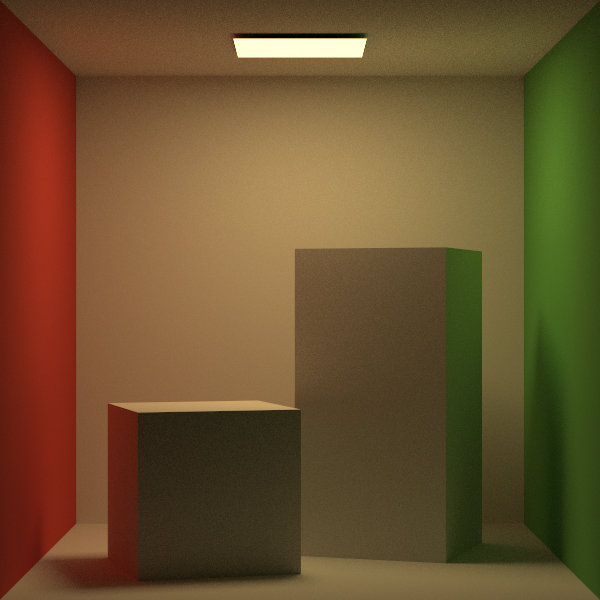
\includegraphics[width=0.45\textwidth]{"/home/lee/Desktop/CG/PA4/report/images/simple.png"}
	\caption{simple box}
\end{figure}
\begin{figure}[H]
	\centering
	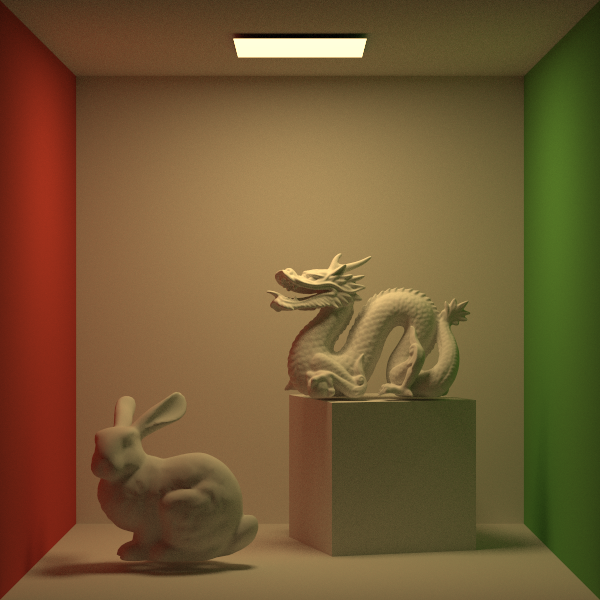
\includegraphics[width=0.45\textwidth]{"/home/lee/Desktop/CG/PA4/report/images/large_mesh.png"}
	\caption{large mesh}
\end{figure}
\begin{figure}[H]
	\centering
	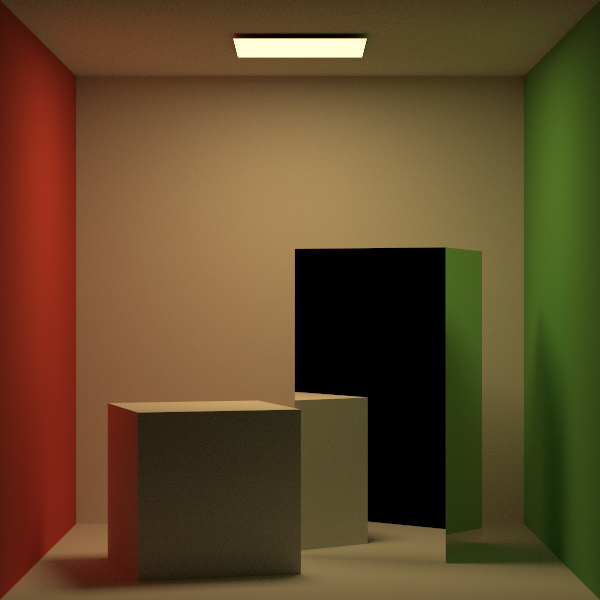
\includegraphics[width=0.45\textwidth]{"/home/lee/Desktop/CG/PA4/report/images/ideal_specular.png"}
	\caption{Ideal specular}
\end{figure}
\begin{figure}[H]
	\centering
	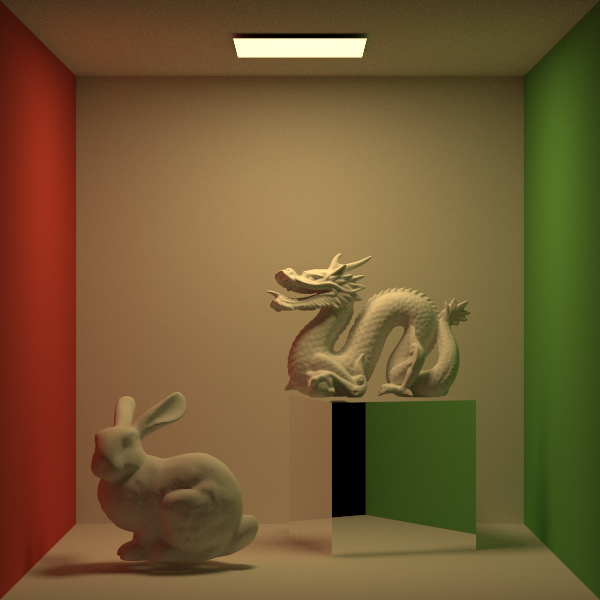
\includegraphics[width=0.45\textwidth]{/home/lee/Desktop/CG/PA4/report/images/specualr_large_mesh.png}
	\caption{large mesh with specular brdf}
\end{figure}
\end{document}
